% !TEX TS-program = pdflatex
% !TEX encoding = UTF-8 Unicode

% This is a simple template for a LaTeX document using the "article" class.
% See "book", "report", "letter" for other types of document.

\documentclass[11pt]{article} % use larger type; default would be 10pt

\usepackage[utf8]{inputenc} % set input encoding (not needed with XeLaTeX)

%%% Examples of Article customizations
% These packages are optional, depending whether you want the features they provide.
% See the LaTeX Companion or other references for full information.

%%% PAGE DIMENSIONS
\usepackage{geometry} % to change the page dimensions
\geometry{a4paper} % or letterpaper (US) or a5paper or....
% \geometry{margin=2in} % for example, change the margins to 2 inches all round
% \geometry{landscape} % set up the page for landscape
%   read geometry.pdf for detailed page layout information

\usepackage{graphicx} % support the \includegraphics command and options

% \usepackage[parfill]{parskip} % Activate to begin paragraphs with an empty line rather than an indent

%%% PACKAGES
\usepackage{booktabs} % for much better looking tables
\usepackage{array} % for better arrays (eg matrices) in maths
\usepackage{paralist} % very flexible & customisable lists (eg. enumerate/itemize, etc.)
\usepackage{verbatim} % adds environment for commenting out blocks of text & for better verbatim
\usepackage{subfig} % make it possible to include more than one captioned figure/table in a single float
\usepackage{cite}
% These packages are all incorporated in the memoir class to one degree or another...

%%% HEADERS & FOOTERS
\usepackage{fancyhdr} % This should be set AFTER setting up the page geometry
\pagestyle{fancy} % options: empty , plain , fancy
\renewcommand{\headrulewidth}{0pt} % customise the layout...
\lhead{}\chead{}\rhead{}
\lfoot{}\cfoot{\thepage}\rfoot{}

%%% SECTION TITLE APPEARANCE
\usepackage{sectsty}
\allsectionsfont{\sffamily\mdseries\upshape} % (See the fntguide.pdf for font help)
% (This matches ConTeXt defaults)

\usepackage{authblk} %Allow more complex author information

%%% ToC (table of contents) APPEARANCE
\usepackage[nottoc,notlof,notlot]{tocbibind} % Put the bibliography in the ToC
\usepackage[titles,subfigure]{tocloft} % Alter the style of the Table of Contents
\renewcommand{\cftsecfont}{\rmfamily\mdseries\upshape}
\renewcommand{\cftsecpagefont}{\rmfamily\mdseries\upshape} % No bold!

%%% END Article customizations

%%% The "real" document content comes below...

\title{A Game Theoretical Exploration of Open Science}
\author[1]{Robert Olendorf}
\author[2]{Steve Koch}
\affil[1]{University Libraries, University of New Mexico}
\affil[2]{Department of Physics and Astronomy, University of New Mexico}
%\date{} % Activate to display a given date or no date (if empty),
         % otherwise the current date is printed 

\begin{document}
\maketitle

%\section{}

The value of sharing data and other research products is increasingly recognized. Many funding agencies, such as NSF and NIH now require that data created through their grants be made available to others in a reasonable amount of time. Additionally, many journals now require or encourage that the data used as a basis for a manuscript be made available. Universities, including University of New Mexico, are working to create data repositories to help researchers make the products of their research available. 

While acknowledging the public good of making their data more avaialble, many if not most individual researchers are still reluctant to make their data available. There are several reasons for this attitude. First and foremost is researchers fear that others will publish from their data before them. Additionally, researchers worry that their data will be used without proper attribution and that their data will be misunderstood or used inappropriately. Essentially, researchers believe that while making their data more open may benefit society, there are few personal benefits and considerable personal risks to doing so. This dichotomy between the wish to make research more open for the public good, and to keep data closed for personal interest creates a tension between funding agencies, policy makers and others hoping to make research more open, and individual researchers who create the content.

In this manuscript we will use game theoretical arguments, specifically work based on the well researched Prisoners' Dilemma to explore how we can create an atmosphere where researchers feel they receive direct benefits to making their data more open. We will show that it is possible that even in the current environment openness in research direclty benefits researchers. We will also explore ways to further increase direct benefits to researchers. Finally, we will provide examples from our own experiences in open research, as well as experimental examples from the literature that show how openness can be encouraged.
\section{The Prisoners' Dilemma}
We will use the Prisoners' Dilemma to explore open science. The Prisoners' Dilemma is a game theoretical construct developed in the RAND corporation by Merrill Flood and Melving Dresher in 1950 \cite{ABAGFBEC19920101, unm.b196052419570101} to study situations where there is both a strong incentive to cooperate, but also a strong temptation to defect. Figure~\ref{pdmatrix} shows a specific example of the Prisoners' Dilemma (PD). In the PD each player can do one of two actions, Cooperate, or Defect (cheat). Cooperating yields a relatively high reward. However, if a player can defect while the other player cooperates, they get an even higher reward. 

If the game is to be played only once, then the only rational move is to defect. If Player 1 knows that Player 2 will cooperate, then she maximizes her reward by defecting and yielding 10. On the other hand, if Player 1 knows that Player 2 will defect, then she should still defect because then she will get at least 3 rather than 0. Player 2 follows the same logic and the equilibrium is for both players to defect. This is known as a Nash Equilibrium, defined as a situation when neither player benefits by changing strategies \cite{unm.b196052419570101}.

If the game is to played for some unknown number of times, then the situation becomes much more complicated. 

\begin{figure}
	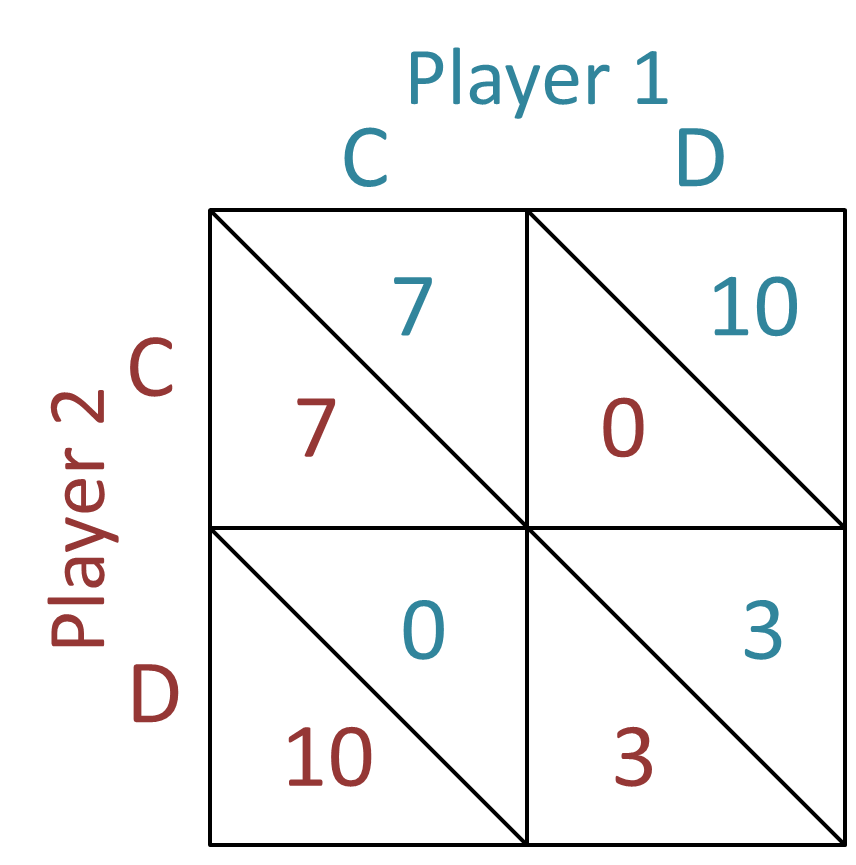
\includegraphics[width=0.5\textwidth]{pdmatrix.png}
	\caption{A sample example matrix for the Prisoners' Dilemma. The players can either Cooperate(C) or Defect(D).  Numbers above the diagonal represent payoffs to Player 1, numbers below the diagonal represent payoffs to Player 2.}
	\label{pdmatrix}
\end{figure}

\bibliographystyle{plain}

\bibliography{refs}
\end{document}
